%%
%% This is file `sample-manuscript.tex',
%% generated with the docstrip utility.
%%
%% The original source files were:
%%
%% samples.dtx  (with options: `all,proceedings,bibtex,manuscript')
%% 
%% IMPORTANT NOTICE:
%% 
%% For the copyright see the source file.
%% 
%% Any modified versions of this file must be renamed
%% with new filenames distinct from sample-manuscript.tex.
%% 
%% For distribution of the original source see the terms
%% for copying and modification in the file samples.dtx.
%% 
%% This generated file may be distributed as long as the
%% original source files, as listed above, are part of the
%% same distribution. (The sources need not necessarily be
%% in the same archive or directory.)
%%
%%
%% Commands for TeXCount
%TC:macro \cite [option:text,text]
%TC:macro \citep [option:text,text]
%TC:macro \citet [option:text,text]
%TC:envir table 0 1
%TC:envir table* 0 1
%TC:envir tabular [ignore] word
%TC:envir displaymath 0 word
%TC:envir math 0 word
%TC:envir comment 0 0
%%
%%
%% The first command in your LaTeX source must be the \documentclass
%% command.
%%
%% For submission and review of your manuscript please change the
%% command to \documentclass[manuscript, screen, review]{acmart}.
%%
%% When submitting camera ready or to TAPS, please change the command
%% to \documentclass[sigconf]{acmart} or whichever template is required
%% for your publication.
%%
%%
\documentclass[manuscript,screen,review]{acmart}

\usepackage{caption}
\usepackage[utf8]{inputenc}
\usepackage[capitalize, noabbrev]{cleveref}
\usepackage{enumitem}

%%
%% \BibTeX command to typeset BibTeX logo in the docs
\AtBeginDocument{%
  \providecommand\BibTeX{{%
    Bib\TeX}}}

%% Rights management information.  This information is sent to you
%% when you complete the rights form.  These commands have SAMPLE
%% values in them; it is your responsibility as an author to replace
%% the commands and values with those provided to you when you
%% complete the rights form.
\setcopyright{acmlicensed}
\copyrightyear{2024}
\acmYear{2024}
\acmDOI{XXXXXXX.XXXXXXX}

%% These commands are for a PROCEEDINGS abstract or paper.
\acmConference[Koli Calling '24]{24th Koli Calling International Conference on Computing Education Research}{November 14--17,
  2024}{Koli, Finland}
%%
%%  Uncomment \acmBooktitle if the title of the proceedings is different
%%  from ``Proceedings of ...''!
%%
%%\acmBooktitle{Woodstock '18: ACM Symposium on Neural Gaze Detection,
%%  June 03--05, 2018, Woodstock, NY}
% \acmISBN{978-1-4503-XXXX-X/18/06}


%%
%% Submission ID.
%% Use this when submitting an article to a sponsored event. You'll
%% receive a unique submission ID from the organizers
%% of the event, and this ID should be used as the parameter to this command.
%%\acmSubmissionID{123-A56-BU3}

%%
%% For managing citations, it is recommended to use bibliography
%% files in BibTeX format.
%%
%% You can then either use BibTeX with the ACM-Reference-Format style,
%% or BibLaTeX with the acmnumeric or acmauthoryear sytles, that include
%% support for advanced citation of software artefact from the
%% biblatex-software package, also separately available on CTAN.
%%
%% Look at the sample-*-biblatex.tex files for templates showcasing
%% the biblatex styles.
%%

%%
%% The majority of ACM publications use numbered citations and
%% references.  The command \citestyle{authoryear} switches to the
%% "author year" style.
%%
%% If you are preparing content for an event
%% sponsored by ACM SIGGRAPH, you must use the "author year" style of
%% citations and references.
%% Uncommenting
%% the next command will enable that style.
%%\citestyle{acmauthoryear}


%%
%% end of the preamble, start of the body of the document source.
\begin{document}

%%
%% The "title" command has an optional parameter,
%% allowing the author to define a "short title" to be used in page headers.
% \title{Automated Feedback Loops: Enhancing Student Motivation and Performance in Programming Courses}
\title{Direct automated feedback delivery for student submissions based on LLMs}

%%
%% The "author" command and its associated commands are used to define
%% the authors and their affiliations.
%% Of note is the shared affiliation of the first two authors, and the
%% "authornote" and "authornotemark" commands
%% used to denote shared contribution to the research.


\author{Maximilian Sölch}
\email{maximilian.soelch@tum.de}
\orcid{0009-0004-1509-7842} 
\affiliation{%
	\institution{Technical University of Munich}
	\city{Munich}
	\country{Germany}
}

\author{Felix T.J. Dietrich}
\email{felixtj.dietrich@tum.de}
\orcid{0009-0007-5826-2061} 
\affiliation{%
	\institution{Technical University of Munich}
	\city{Munich}
	\country{Germany}
}

\author{Stephan Krusche}
\email{krusche@tum.de}
\orcid{0000-0002-4552-644X}
\affiliation{%
	\institution{Technical University of Munich}
	\city{Munich}
	\country{Germany}
}

%%
%% By default, the full list of authors will be used in the page
%% headers. Often, this list is too long, and will overlap
%% other information printed in the page headers. This command allows
%% the author to define a more concise list
%% of authors' names for this purpose.
\renewcommand{\shortauthors}{Sölch et al.}

%%
%% The abstract is a short summary of the work to be presented in the
%% article.
\begin{abstract}

  Receiving timely and personalized feedback is crucial for students' learning progress and motivation. 
  However, providing such feedback poses a significant challenge in education, particularly as student numbers have steadily increased in recent years.
  This growth has made it difficult for tutors and professors to deliver individualized feedback to each student, resulting in a time-consuming, repetitive, and often manual task that contributes to a heavy workload for educators.

  This paper presents DAFeeD, a large language model (LLM)-based approach for providing automated formative feedback on student submissions.
  The exercise-independent approach can be applied to various domains, such as programming, text, or modeling exercises. 
  By incorporating exercise-specific information, such as the problem statement and grading instructions, into the prompt, the feedback is tailored to the exercise context.
  
  We implemented this approach in an open-source reference implementation named Athena, which is integrated with the learning platform Artemis.
  To evaluate the effectiveness and efficiency of the approach, we conducted a controlled study with students.
  The results show ... %todo: add results

\end{abstract}

%%
%% The code below is generated by the tool at http://dl.acm.org/ccs.cfm.
%% Please copy and paste the code instead of the example below.
%%
\begin{CCSXML}
  <ccs2012>
     <concept>
         <concept_id>10003456.10003457.10003527.10003540</concept_id>
         <concept_desc>Social and professional topics~Student assessment</concept_desc>
         <concept_significance>500</concept_significance>
         </concept>
     <concept>
         <concept_id>10010405.10010489</concept_id>
         <concept_desc>Applied computing~Education</concept_desc>
         <concept_significance>500</concept_significance>
         </concept>
   </ccs2012>
\end{CCSXML}
  
\ccsdesc[500]{Social and professional topics~Student assessment}
\ccsdesc[500]{Applied computing~Education}

%%
%% Keywords. The author(s) should pick words that accurately describe
%% the work being presented. Separate the keywords with commas.
\keywords{Do, Not, Us, This, Code, Put, the, Correct, Terms, for,
  Your, Paper}

% \received{20 February 2007}
% \received[revised]{12 March 2009}
% \received[accepted]{5 June 2009}

%%
%% This command processes the author and affiliation and title
%% information and builds the first part of the formatted document.
\maketitle

\section{Introduction} % 1 page

% problem
% time consuming, not scalable, not always available
% hinders learning progress and motivation %todo: reference for this!

% todo: reference for this!
In the current educational landscape, providing timely and effective feedback to students remains a significant challenge.
Traditionally, students must wait for course tutors or professors to review their submissions and provide feedback.
This process can be time-consuming, often requiring students to arrange meetings and wait for available time slots, which are not always convenient or immediate.
Similar it is timecosuming and tedious for professors and tutors to provide asynchronous feedback via email or other communication channels.
The inherent delays and scheduling difficulties make this approach not scalable, especially in courses with a large number of students.

%todo: interactive learning concept (ref stephans paper)
% todo: reference for this!
These limitations hinder students' learning progress and motivation.
The waiting period for feedback interrupts the learning flow, causing students to lose momentum and potentially disengage from the subject matter.
%todo: reference for this!
Additionally, the limited availability of tutors and professors means that not all students receive the individualized attention they need to improve their understanding and skills.
This situation underscores the necessity for a more efficient and scalable feedback system that can provide continuous support to students without the constraints of traditional methods.


% Objectives
In this paper, we present an approach for generating automated feedback on student submissions using large language models (LLMs) to address these challenges.
The approach is independent of the exercise type and can be applied to various domains, such as programming, text, or modeling exercises.
We implemented the approach in an open-source reference implementation called Athena, connected to the learning platform Artemis through which students submit their solutions and receive feedback.
To validate the effectiveness and efficiency of the approach, we tested it in a controlled environment. 
We collected quantitative and qualitative data to evaluate students' perceptions of the approach and the overall performance of the reference implementation.
The results show %todo: add results


%Outline
The subsequent sections of this paper are organized to provide a comprehensive understanding of the research. 
\cref{sec:related-work} provides an overview of related work. 
\cref{sec:approach:DAFeeD} details the concept and methodology of Direct Automated Feedback Delivery (DAFeeD).
\cref{sec:reference-implementation} describes the reference implementation of DAFeeD, called Athena, including a general overview, details on the used prompts, and the system architecture. 
\cref{sec:evaluation} presents the evaluation results, %todo: add results 
Finally, \cref{sec:conclusion} concludes with a summary of findings and discusses future research directions to enhance automated feedback systems.

\newpage
\section{Related Work} % 2 page
\label{sec:related-work}

The necessity and challenges of providing effective feedback in educational settings have been widely recognized. This section overviews prior work in three interrelated areas: automated feedback systems, the application of large language models in educational feedback, and feedback delivery mechanisms within learning platforms.

\subsection{Automated Feedback Systems}

todo
\cite{hahn:2021:SystematicReviewEffects}

\subsection{Large Language Models in Educational Feedback}

\subsection{Feedback Delivery in Learning Platforms}

% AI Teaches the Art of Elegant Coding: Timely, Fair, and Helpful Style Feedback in a Global Course
% SIGCSE 2024
% Citations: 0 (1 on google), 164 downloads on ACM
% \cite{woodrow:2024:AITeachesArta}
%
%%%% Related work: 
%%%% - Timeliness of feedback:
%%%% 1. James A. Kulik and Chen-Lin C. Kulik. 1988. Timing of Feedback and Verbal Learning. Review of Educational Research 58 (1988), 79 – 97. https: //api.semanticscholar.org/CorpusID:145572756
%%%% 2. Kathryn Haughney, Shawnee Wakeman, and Laura Hart. 2020. Quality of Feedback in Higher Education: A Review of Literature. Education Sciences 10, 3 (2020). https://doi.org/10.3390/educsci10030060
%%%% 3. John C. Chen, Dexter C. Whittinghill, and Jennifer A. Kadlowec. 2006. Using Rapid Feedback to Enhance Student Learning and Satisfaction. In Proceedings. Frontiers in Education. 36th Annual Conference. 13–18. https://doi.org/10.1109/ FIE.2006.322306
%%%% 4. D.S. Goldstein, J.W. Pellegrino, S.R. Goldman, T.M. Stoelinga, N.T. Heffernan, and C. Heffernan. 2016. Improving mathematical learning outcomes through applying principles of spaced practice and assessment with feedback. Poster presented at the Annual Meeting of the American Educational Research Association.
%%%%
%%%% - Automated feedback tools:
%%%% mostly on style feedback (static analysis, rule-based tools)
%%%% More modern tools NLP (clustering using pre-existing solutions)
%%%% No LLM based tools as related work and it is 2024...


% CodeHelp: Using Large Language Models with Guardrails for Scalable Support in Programming Classes
% Koli Calling '23 
% Citations: 45
% \cite{liffiton:2024:CodeHelpUsingLarge}
%
% In our work, students receive immediate feedback from CodeHelp at any time of the day or night.
%
%%%% Related Work:
%%%% Too much, they have 20-30 references in the related work section
%%%%
%%%% Key differences pointed out to:
%%%% 1. (see below Koli '23) Majeed Kazemitabaar, Justin Chow, Carl Ka To Ma, Barbara J. Ericson, David Weintrop, and Tovi Grossman. 2023. Studying the Effect of AI Code Generators on Supporting Novice Learners in Introductory Programming. In Proceedings of the 2023 CHI Conference on Human Factors in Computing Systems (Hamburg, Germany) (CHI ’23). Association for Computing Machinery, New York, NY, USA, Article 455, 23 pages. https://doi.org/10.1145/3544548.3580919
%%%% 2. (see below ICER '23)  Arto Hellas, Juho Leinonen, Sami Sarsa, Charles Koutcheme, Lilja Kujanpää, and Juha Sorva. 2023. Exploring the Responses of Large Language Models to Beginner Programmers’ Help Requests. arXiv:2306.05715 [cs.CY]

% How Novices Use LLM-based Code Generators to Solve CS1 Coding Tasks in a Self-Paced Learning Environment
% Koli Calling '23
% Citations: 37
% \cite{kazemitabaar:2024:HowNovicesUse}
%
%%%% Related Work:
%%%%
%%%% - Programmers’ Experience with AI Coding Assistants
%%%% ...
%%%% - Large Language Models in Computer Science Education
%%%% ...


% Exploring the Responses of Large Language Models to Beginner Programmers’ Help Requests
% ICER '23
% Citations 5 on ACM 68 on google, 834 downloads
% \cite{hellas:2023:ExploringResponsesLargea}
%
%%%% No obvious related work section, besides background


% Using GPT-4 to Provide Tiered, Formative Code Feedback
% SIGCSE 2024
% Citations: 0 (rather new), 260 downloads on ACM
% \cite{nguyen:2024:UsingGPT4Provide}
%
%%%% Related Work:
%%%%
%%%% - Automated formative feedback
%%%% ...
%%%% - Potential of Large Language Models
%%%% ...


% Using Large Language Models to Enhance Programming Error Messages
% SIGCSE 2023
% Citations: 61 (119 on google), 2607 downloads on ACM
% \cite{leinonen:2023:UsingLargeLanguagea}
%
%%%% Related Work / Background:
%%%%
%%%% - Programming Error Messages
%%%% ...
%%%% - Large Language Models
%%%% ...


% Next-Step Hint Generation for Introductory Programming Using Large Language Models
% ACE '24
% Citations: 1 on ACM (5 on Google), 163 downloads on ACM
% \cite{roest:2024:NextStepHintGeneration}
%%%% Related Work:
%%%%
%%%% - Automated feedback
%%%%   - Providing effective feedback.
%%%%   - Feedback on programming tasks.
%%%%   - Data-driven next-step hints.
%%%%
%%%% - Large language models
%%%%   - LLM in programming education.

\newpage
\section{Approach: Direct Automated Feedback Delivery (DAFeeD)} % 1 page
\label{sec:approach:DAFeeD}

DAFeeD employs large language models to deliver automated feedback on student submissions, designed to complement traditional teaching methods and provide additional support.
Figure \ref{fig:DAFeeD-workflow} illustrates the continuous feedback workflow that DAFeeD facilitates, enabling students to receive feedback at any time, thereby eliminating the need to wait for responses from human tutors or course professors.

\begin{figure}[htbp]
  \centering
  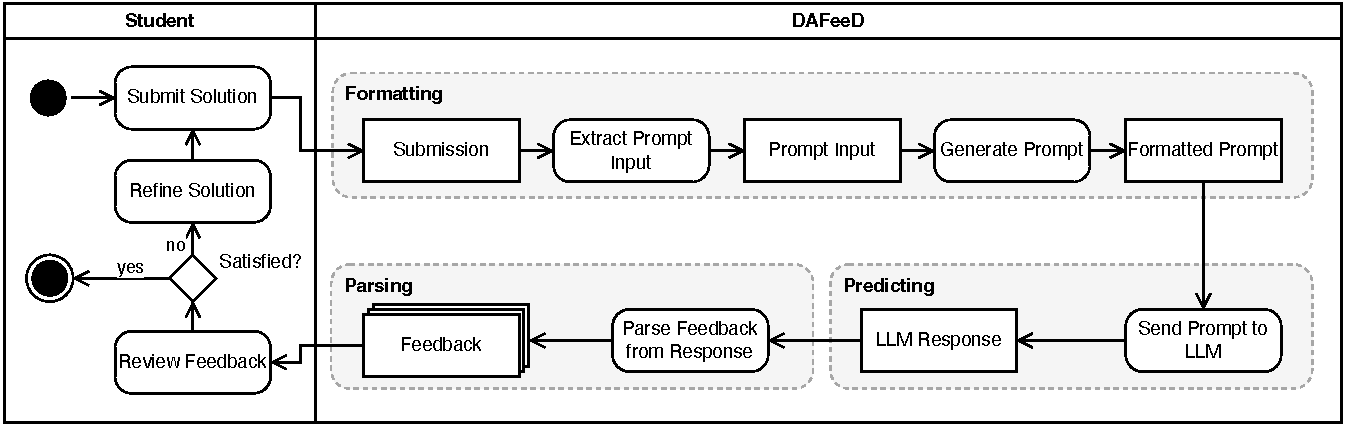
\includegraphics[width=\linewidth]{figures/DAFeeD-ActivityDiagram.pdf}
  \caption{Workflow of direct automated feedback delivery for students' submissions (UML Activity Diagram)}
  \label{fig:DAFeeD-workflow}
\end{figure}

%todo: exercise independent
DAFeeD can provide feedback on various aspects, such as the correctness of the code, the quality of the code, and the performance of the student.
Once the student submits their solution, DAFeeD initiates a three-stage process to generate natural language feedback.

%todo: add learner profile (find reference) to generate individualized, personal feedback tailored to the student's learning progress and needs.
The first stage, called \textit{Formatting}, takes the student's submission and extracts the submission content, problem statement including learning objectives, and any possible grading instructions the instructor defines.
This extracted information represents the prompt input.
During the prompt generation step, a predefined prompt template is filled with the prompt input data, resulting in a formatted prompt.

In the second stage, called \textit{Predicting}, the formatted prompt is sent to a large language model (LLM), which generates a response that includes detailed feedback for the student.

The final stage, \textit{Parsing}, takes the LLM response, which comes in the JSON format, and parses feedback items from it. 
In addition to the feedback text, the feedback object also contains reference information indicating the part of the submission it pertains to.
For programming exercises, this includes the file name and line number of the relevant code snippet to which the feedback refers.
For text exercises, the reference information includes only the sentence or word range the feedback refers to.

All of the feedback is then returned to the student for review.
If the student is satisfied with the feedback, the process concludes. 
Otherwise, the student can refine their solution and resubmit it, initiating the DAFeeD process anew.

This iterative process is designed to motivate students to continuously learn and experiment with their solutions, resulting in improved performance.


\section{Reference Implementation: Athena} % 2 pages
\label{sec:reference-implementation}

We incorporated DAFeeD into a reference implementation named Athena, which is seamlessly integrated with the learning platform Artemis. 
Through Artemis, students can submit their solution and review the feedback.

When submitting their solutions on Artemis, students have the option to request direct automated feedback by clicking a newly added button.
This feedback request is then sent to Athena, provided the student has not reached their feedback request limit for the exercise.
Course instructors can customize the number of allowed feedback requests per exercise according to their preference.
A status visualization informs students about their feedback request state.
Once Athena generates the feedback and sends it back to Artemis, the student can review it in a modal window on Artemis, as depicted in Figure \ref{fig:Artemis-feedback-visualization}.

%todo: find better example for feedback including a positive feedback feedback item
\begin{figure}[htbp]
  \centering
  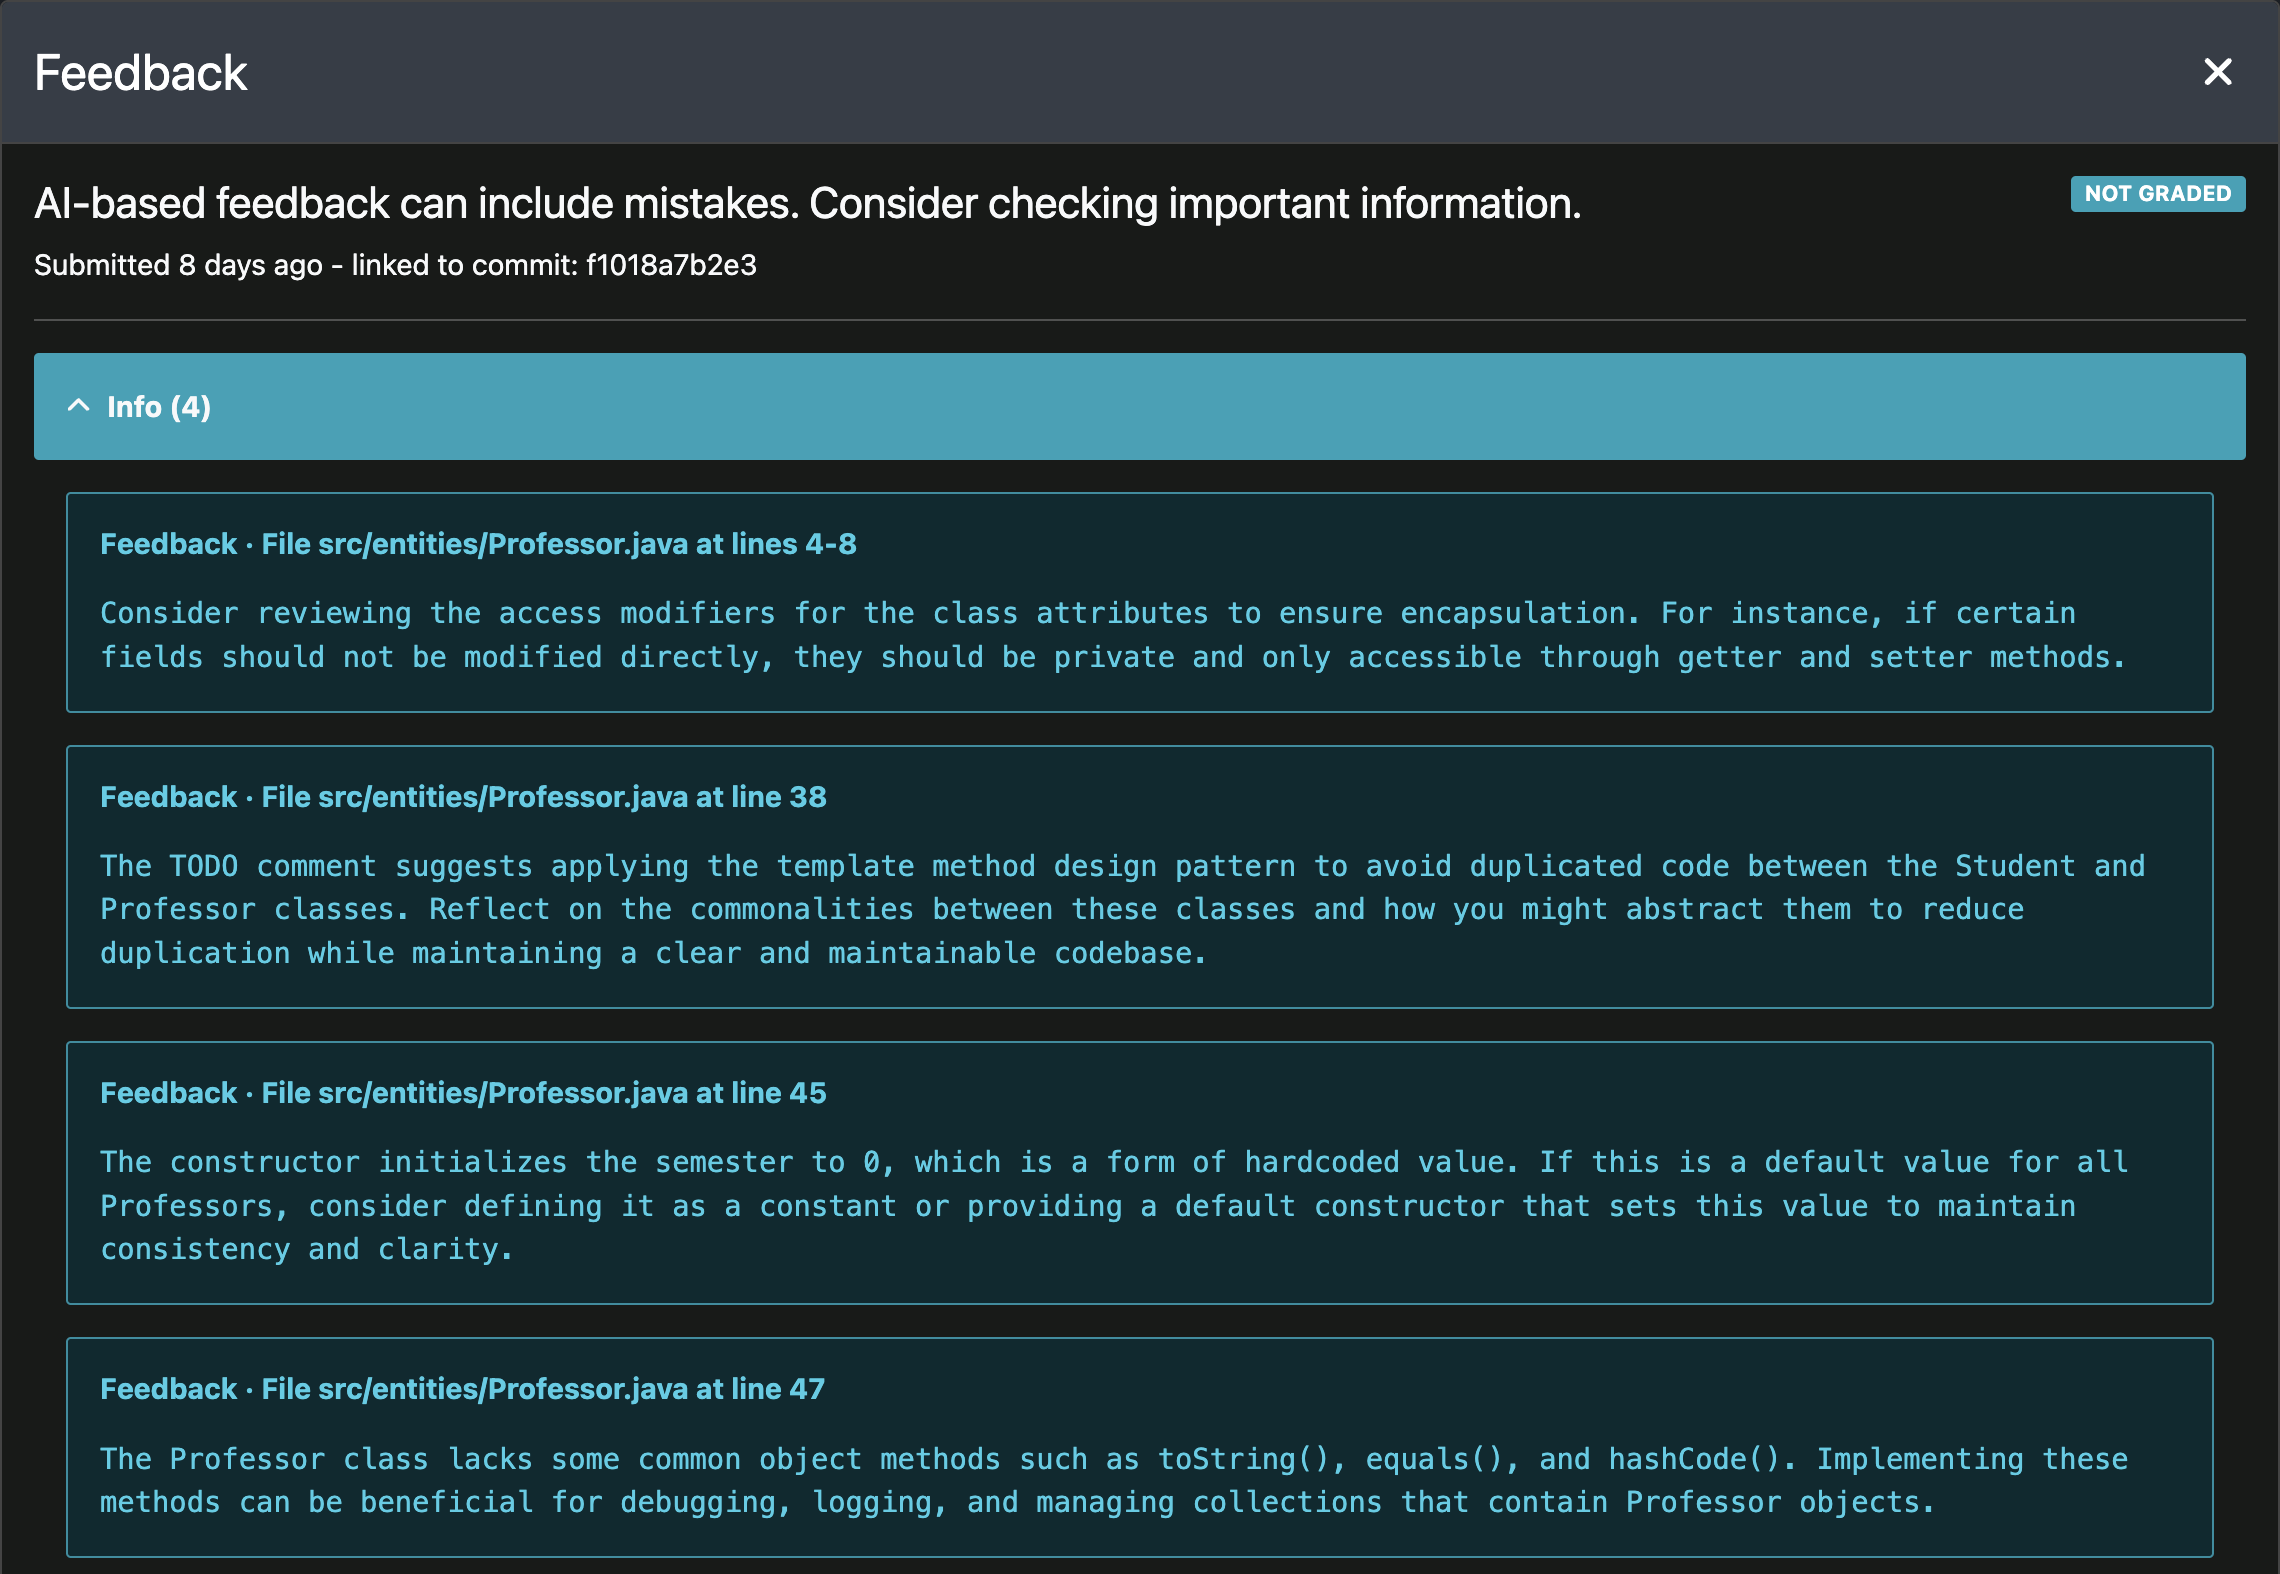
\includegraphics[width=0.9\linewidth]{figures/artemis-feedback_anonymized.png}
  \caption{Visualization of the feedback how students see it in Artemis.}
  \label{fig:Artemis-feedback-visualization}
\end{figure}

\subsection{Prompts}

%Todo: Listing of the used prompt (at least simplified) and an explanation of the prompt

\subsection{Feedback Generation}

\subsection{Architecture}

Athena is deployed in production alongside the learning platform Artemis, which serves up to more than 2000 students per course.
Consequently, the reference implementation must satisfy additional non-functional requirements such as performance, scalability, maintainability, and usability.
To meet these requirements and to support feedback generation for multiple exercise types while allowing for future extensibility, we adopted a modular architecture, as illustrated in Figure \ref{fig:Athena-architecture}.

%TODO: anonymize the figure (Artemis, Athena )
\begin{figure}[htbp]
  \centering
  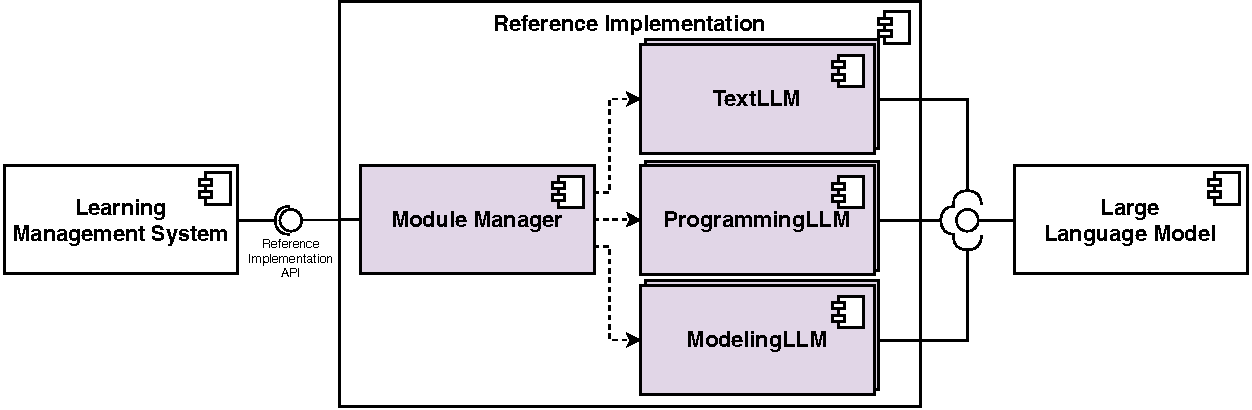
\includegraphics[width=\linewidth]{figures/Athena-Architecture.pdf}
  \caption{Top Level Archietecture of the reference implementation Athena (UML Deployment Diagram)}
  \label{fig:Athena-architecture}
\end{figure}

The \textit{Module Manager} handles all incoming requests, verifies authorization, and forwards them to the appropriate modules.
The \textit{ProgrammingLLM} module manages programming exercises and executes the three-stage DAFeeD process, which includes formatting, predicting, and parsing. 
Similarly, the \textit{TextLLM} module is optimized for text exercises and follows the same process.

Athena's system design is independent of any specific learning management system (LMS) as it provides a REST API, documented using the OpenAPI standard\footnote{\url{https://www.openapis.org}}.
This independence allows Athena to be integrated with various LMS platforms, such as Moodle\footnote{\url{https://moodle.org}}.

Athena currently connects to OpenAI models hosted in a private Azure cloud to ensure that student data is not used for training models, maintaining privacy.
Additionally, the system can be configured to use open-source models like Llama\footnote{\url{https://llama.meta.com}} or Mistral\footnote{\url{https://mistral.ai}}, either self-hosted or cloud-based.

To meet performance and scalability requirements, Athena and its modules are deployed within a Kubernetes cluster\footnote{\url{https://kubernetes.io}}.
Kubernetes, in conjunction with Athena's modular architecture, allows the system to scale each module independently.
For example, additional instances of the programming module can be instantiated when a new programming exercise is released.
Furthermore, Kubernetes provides out-of-the-box load balancing and self-healing capabilities, ensuring that if a module crashes, it is automatically restarted.


\section{Evaluation} % 5 pages
\label{sec:evaluation}

In this section, we outline the methodology employed to validate the effectiveness of the proposed DAFeeD approach including the reference implementation Athena.
The conducted evaluation represents the treatment validation stage of the design science methodology proposed by Wieringa \cite{wieringa:2014:DesignScienceMethodologya}.
In this stage, the proposed solution — DAFeeD — is evaluated in a controlled environment, and the collected data is utilized for the refinement and improvement of the solution.

We begin by describing the research questions, followed by the study design and the results.
Subsequently, we outline the limitations of the evaluation and discuss the implications of the findings.


\subsection{Research Questions}

With this study, we want to answer the following research questions about direct automated feedback delivery:

\begin{enumerate}[label=\textbf{RQ\arabic*}]
  \item How do students perceive the effectiveness of direct automated feedback?
  \item How does the availability of direct automated feedback affect student engagement and motivation?
  \item Do students feel more comfortable requesting automatic feedback than asking a human tutor or the course professor?
  \item How do students perceive the usability and helpfulness of DAFeeD?
\end{enumerate}

%todo: describe research questions


\subsection{Study Design}
To gain comprehensive insights into students' perceptions of the newly introduced DAFeeD concept, we employed a survey-based approach.
Initially, study participants tested the new feedback feature on a sample exercise using the Artemis platform in a controlled environment at the university.
The study conductors were present throughout to answer questions and provide support as needed.
Following this hands-on experience, participants were asked to complete a survey hosted on the community version of the open-source survey tool LimeSurvey\footnote{\url{https://www.limesurvey.org}}.
This survey aimed to gather their opinions on direct automated feedback and collect feedback on their overall experience with the feature.

We invited students from current courses at the university to participate in the study via direct messages and conducted the study with a total of 20 participants.
The study uses a mixed methods approach, combining quantitative and qualitative data collection methods. 
The participants were a mix of undergraduate and graduate students from various disciplines, including computer science, information systems, and games engineering.
%todo: describe participants 
%todo: cite nielsen regarding number of participants

%todo: describe survey
%likert scale, open questions
All survey questions, except for the introductory demographic queries and the final, voluntary free-text responses, employ a 5-point Likert scale \cite{allen:2007:LikertScalesData} and are mandatory.
%Question Group 1
The survey commences with a series of introductory demographic inquiries, including the student's current study program, ongoing degree pursued, and academic semester. 
Additionally, respondents are asked to provide information regarding the hardware employed, including details on the operating system and web browser used.
The final question in this group asks participants to describe their programming experience.

%Question Group 2
Following the demographic section, the survey explores participants' opinions on the impact of direct automated feedback on student engagement and motivation.
%Question Group 3
Subsequently, the survey queries participants on their comfort with the feedback source, specifically whether they prefer receiving feedback from a human tutor or from the DAFeeD feature.
%Question Group 4
The survey then investigates aspects related to participants' perceived effectiveness of the DAFeeD feature.
%Question Group 5
In the final question group, participants assess the overall usability and helpfulness of the DAFeeD feature.

\subsection{Results}

\subsection{Limitations}

\subsection{Discussion}


\section{Conclusion \& Future Work} % 1 page
\label{sec:conclusion}

%future work
% 
Future work includes enhancing the visualization of feedback, such as grouping and color coding the feedback items to make it easier to differentiate between critical feedback items, suggestions for improvement, and positive feedback.
A high priority will be on further improving the overall quality of the feedback provided. 
We also aim to extend the implementation to support direct automated feedback for the remaining exercise types of Artemis.
Another crucial step is to test direct automated feedback in a real-world setting by utilizing this feature in an actual course. 
This will allow us to collect comprehensive data to thoroughly evaluate the impact on student performance and motivation.


%%
%% The next two lines define the bibliography style to be used, and
%% the bibliography file.
\bibliographystyle{ACM-Reference-Format}
\bibliography{main}

\end{document}
\endinput
%%